\begin{surferPage}[Singularidad A4++]{Una singularidad $A_4^{++}$}
Como se ha visto, una $A_4^{+-}$ se parece a una $A_2^{+-}$.
Análogamente,
$A_4^{++}$ y $A_2^{++}$ son casi idénticas.
Las siguientes imágenes muestran superficies
    $A_2^{++}$, $A_4^{++}$,$A_2^{+-}$, $A_4^{+-}$:
    \begin{center}
      \vspace*{-0.2cm}
      \begin{tabular}{@{}c@{\ }c@{\ }c@{\ }c@{}}
        \begin{tabular}{@{}c@{}}
          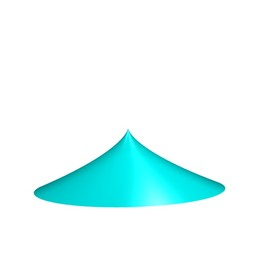
\includegraphics[width=1.2cm]{../../common/images/A2pp}
        \end{tabular}
        &
        \begin{tabular}{@{}c@{}}
          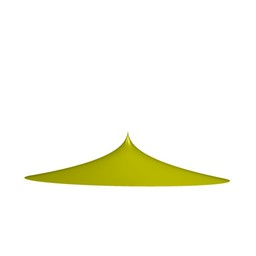
\includegraphics[width=1.2cm]{../../common/images/A4pp}
        \end{tabular}
        &
        \begin{tabular}{@{}c@{}}
          
\includegraphics[width=1.2cm]{../../common/images/A2pm}
        \end{tabular}
        &
        \begin{tabular}{@{}c@{}}
          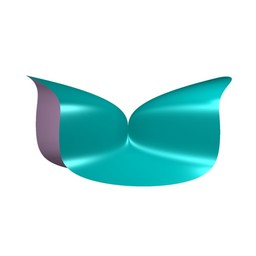
\includegraphics[width=1.2cm]{../../common/images/A4pm}
        \end{tabular}
      \end{tabular}
    \end{center}
    \vspace*{-0.2cm}
Se observa que las superficies
$A_4$ se acercan al punto singular más abruptamente que las $A_2$.

Como en el caso de la $A_4^{+-}$, se obtiene una diferencia crucial
con la $A_2$ solo cuando intentamos deformar la singularidad en
singularidades  cónicas o en una superficie con múltiples agujeros: la
singularidad $A_2^{++}$ solo se puede deformar en una singularidad cónica. Mientras que
$A_4^{++}$ lo hace en dos:
%    \dontshow{
    %
    \begin{center}
      \vspace*{-0.2cm}
      \begin{tabular}{@{}c@{\quad}c@{\quad}c@{}}
        \begin{tabular}{@{}c@{}}
          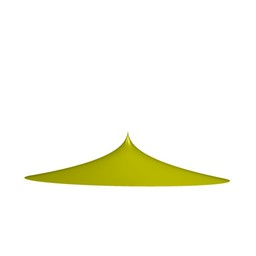
\includegraphics[width=1.2cm]{../../common/images/A4pp_0}
        \end{tabular}
        &
        \begin{tabular}{@{}c@{}}
          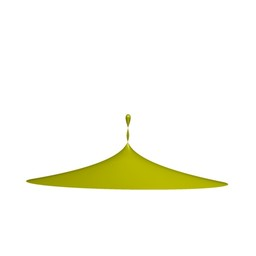
\includegraphics[width=1.2cm]{../../common/images/A4pp_1}
        \end{tabular}
        &
        \begin{tabular}{@{}c@{}}
          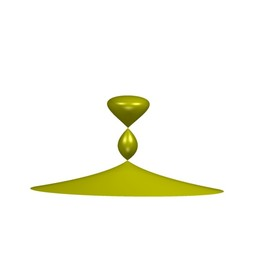
\includegraphics[width=1.2cm]{../../common/images/A4pp_2}
        \end{tabular}
      \end{tabular}
    \end{center}
%    }
      \vspace*{-0.2cm}
Esto se consigue con la ecuación
    \[x^2(x+a^2)^2(x-a^2)+y^2+z^2.\]
 
\end{surferPage}
